\documentclass{article}

\usepackage[top=1in,bottom=1in,right=1in,left=1in]{geometry}
\usepackage[colorlinks=true, urlcolor=blue, linkcolor=violet ]{hyperref}
\usepackage{graphicx}
\usepackage{caption}
\usepackage{listings}
\usepackage{pgfplots}
\usetikzlibrary{calc,angles,quotes}
\usepackage{tikz}
\usepackage{booktabs}
\usepackage[titletoc]{appendix} 
\usepackage{xepersian}
\usepackage{lmodern} 
\usepackage{amsmath}
\usepackage{amssymb}
\usepackage{fancyhdr}
\usepackage{wrapfig} 
\usepackage{mdframed}
\setlength{\emergencystretch}{3em}


\settextfont[Scale=1.1]{XB Niloofar}
\setlatintextfont[Scale=1.0]{Times New Roman}
\setdigitfont[Scale=1.1]{XB Niloofar}


\title{\Large \textbf{آزمایش تداخل دو شکاف یانگ با الکترون‌ها}}
\author{
\begin{minipage}{\textwidth}
\centering
\lr{\textsuperscript{a)} \ \textbf{S. Frabboni}}\\
\lr{\small \textit{Department of Physics, University of Modena and Reggio Emilia and CNR-INFM-S3,}}\\
\lr{\small \textit{Via G. Campi 213/a, 41100 Modena, Italy}}\\[1em]
\textbf{\lr{G. C. Gazzadi}}\\
\lr{\small \textit{CNR-INFM-S3, Via G. Campi 213/a, 41100 Modena, Italy}}\\[1em]
\textbf{\lr{G. Pozzi}}\\
\lr{\small \textit{Department of Physics, University of Bologna, v. B. Pichat 6/2, 40127 Bologna, Italy}}\\[1em]
{\small (دریافت ۳۰ نوامبر ۲۰۰۶؛ پذیرش ۱۴ ژوئن ۲۰۰۷)}
\end{minipage}
}
\date{}

\begin{document}

\twocolumn[
  \maketitle
  \begin{abstract}
  در این یادداشت کوتاه، روشی برای تولید نمونه‌های حاوی دو شکاف در ابعاد نانو گزارش می‌کنیم که برای نمایش آزمایش تداخل الکترون دو شکاف به دانشجویان کارشناسی و تحصیلات تکمیلی در یک میکروسکوپ الکترونی عبوری معمولی مناسب است.
  \end{abstract}
  \vspace{2em}
]

آزمایش تداخل الکترون دو شکاف، که ارزش آموزشی آن در روشن ساختن دوگانگی موج-ذره در فیزیک مدرن غیرقابل انکار است،$^1$ برای مدت طولانی صرفاً به عنوان یک آزمایش ذهنی (gedanken) در نظر گرفته می‌شد.

اولین تحقق واقعی آن توسط Jönsson$^2$ صورت گرفت که با نبوغ خود توانست شکاف‌هایی در محدوده میکرومتر ایجاد کند و آن‌ها را با استفاده از یک دستگاه پراش الکترون اختصاصی که از عدسی‌های الکترواستاتیک استوانه‌ای و متقارن چرخشی تشکیل شده بود، مشاهده کند. این عدسی‌ها برای روشن کردن همدوس شکاف‌ها توسط پرتو الکترونی و بزرگنمایی مناسب الگوی پراش استفاده می‌شدند.

یک نسخه آموزشی جایگزین از آزمایش تداخل دو پرتو، از آنالوگ اپتیک الکترونی منشور دوتایی (biprism) فرنل برای تولید دو منبع همدوس مجازی، به جای منابع واقعی که توسط شکاف‌ها ارائه می‌شوند، استفاده می‌کند. علاوه بر این، پدیده‌های تداخل در ناحیه فرنل (یعنی میدان نزدیک) به جای ناحیه فراونهوفر (یعنی میدان دور) مشاهده می‌شوند.$^{3-5}$

امروزه، پیشرفت‌های فناوری امکان انجام آزمایش یانگ را با استفاده از ابزارهای تجاری فراهم می‌کند: میکروسکوپ الکترونی عبوری (TEM) می‌تواند نقش دستگاه پراش را ایفا کند و یک دستگاه ماشین‌کاری با پرتو یونی متمرکز (FIB) ساخت آسان شکاف‌ها را امکان‌پذیر می‌سازد.$^6$

در این کار ما برخی از نتایج اخیراً به دست آمده را با هدف نشان دادن این آزمایش بنیادی به دانشجویان خود گزارش می‌کنیم، با استفاده از انعطاف‌پذیری اضافی میکروسکوپ‌های الکترونی مدرن که در آن‌ها صفحه عکاسی با یک دوربین دستگاه جفت‌کننده بار (CCD) جایگزین شده است، به طوری که تصاویر می‌توانند به وضوح و مستقیماً در زمان واقعی روی صفحه مانیتور یا حتی روی صفحه نمایش سالن سخنرانی نمایش داده شوند.

شکاف‌ها با استفاده از فرزکاری FIB بر روی یک پنجره غشایی نیترید سیلیکون تجاری که معمولاً برای آماده‌سازی نمونه TEM استفاده می‌شود، ساخته شدند.$^7$ این نمونه از یک قاب سیلیکونی به قطر 3 میلی‌متر و ضخامت 200 میکرومتر، با یک پنجره مربع شکل $100 \times 100\ \mu\text{m}$ در مرکز تشکیل شده است که با یک غشای نیترید سیلیکون به ضخامت 500 نانومتر پوشیده شده است. ضخامت غشا به گونه‌ای انتخاب شد که عبور الکترون از مناطقی غیر از شکاف‌های باز شده به حداقل برسد.

ماشین‌کاری FIB با یک دستگاه پرتو دوگانه (\lr{FEI Strata DB235M}) انجام شد که یک FIB با یون گالیم 30 کیلوالکترون‌ولت را با یک میکروسکوپ الکترونی روبشی \lr{(SEM)} گسیل میدان حرارتی ترکیب می‌کند که دارای وضوح‌های به ترتیب 6 و 2 نانومتر هستند. این سیستم امکان ماشین‌کاری در مقیاس نانو توسط فرزکاری یونی و کنترل همزمان کار در حال انجام توسط تصویربرداری SEM با وضوح بالا را فراهم می‌کند.

 \begin{figure}[h!]
    \centering
    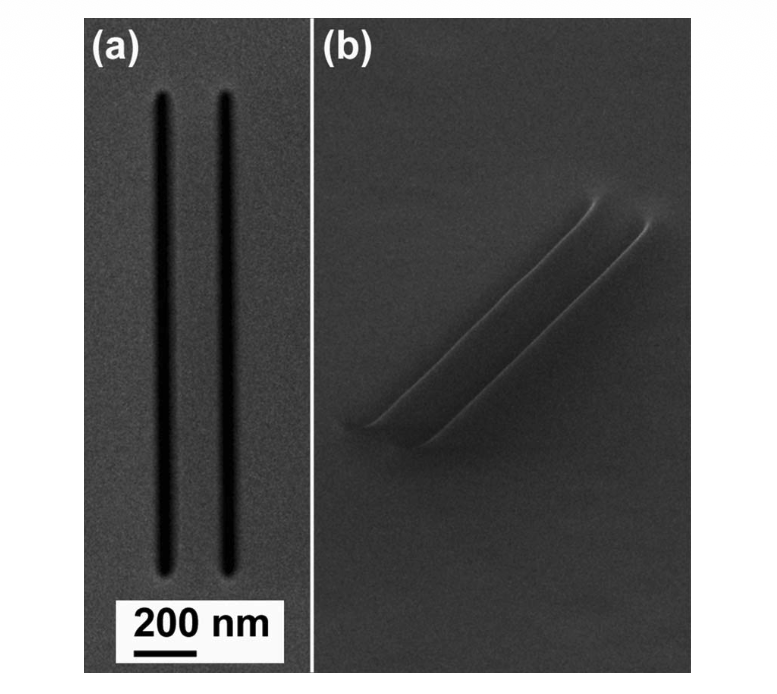
\includegraphics[width=0.5\textwidth]{fig.1.png}
    \caption{تصاویر SEM در نمای روبه‌رو (a) و نمای مایل (b) از شکاف‌های در مقیاس نانو که توسط فرزکاری FIB بر روی یک غشای سیلیکون‌نیتریدی باز شده‌اند}
\end{figure}

 \begin{figure}[h!]
    \centering
    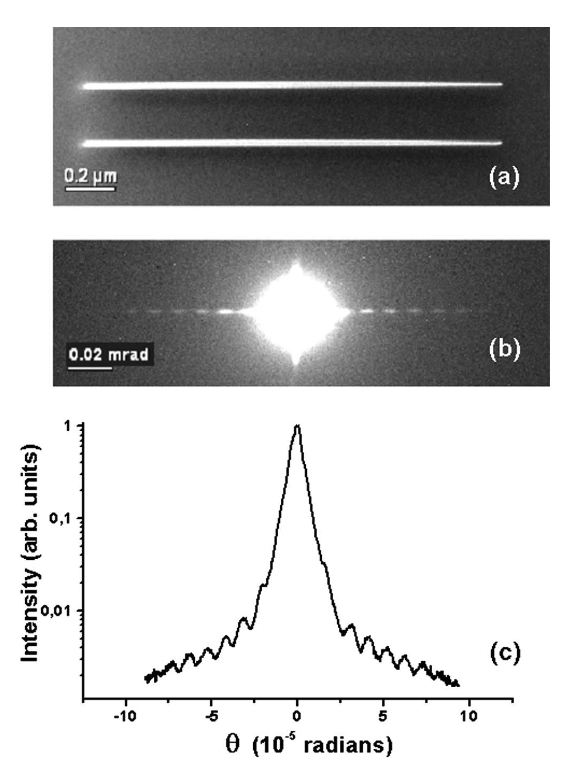
\includegraphics[width=0.5\textwidth]{fig.2.png}
    \caption{(a)تصویر روشن‌میدان TEM از دو شکاف.(b) الگوی پراش الکترونیِ دو شکاف که نسبت به (a) به اندازه‌ی ۹۰ درجه چرخیده است. بیشینه‌های تداخلیِ با فواصل برابر، به وضوح به صورت نوارهای جانبیِ لکه‌ی مرکزیِ اشباع‌شده‌ی انتقال‌یافته قابل مشاهده هستند.(c) نمودارِ لگاریتمیِ شدتِ پراشِ (b) که از پویش خطی با عرض ۵ پیکسلِ طی‌شده بر روی بیشینه‌های تداخلی به دست آمده است.}
\end{figure}

 \begin{figure}[h!]
    \centering
    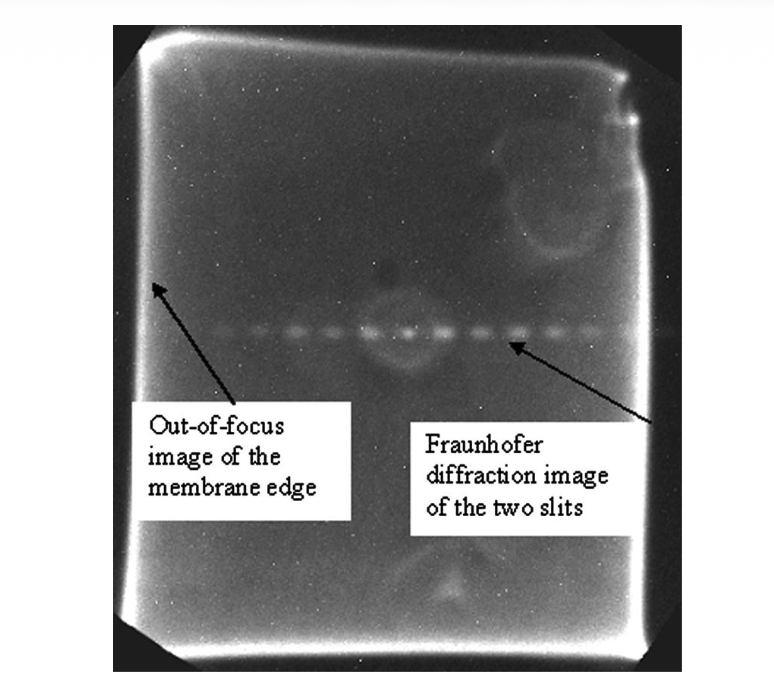
\includegraphics[width=0.5\textwidth]{fig.3.png}
    \caption{تصویر خارج از فوکوسِ الگوی پراش الکترونی، نشان‌داده‌شده در شکل ۲b. ناحیهٔ پهن با کنتراست خاکستری که توسط حاشیهٔ مستطیلیِ روشن در بر گرفته شده است، تصویر خارج از فوکوسِ غشای سیلیکون‌نیترید را نشان می‌دهد؛ در حالی که لکه‌های روشنِ افقی و با فواصل برابر، متناظر با تصویر پراش فراونهوفرِ دو شکاف هستند}
\end{figure}

برای باز کردن شکاف‌ها، یک پرتو \lr{10-pA}، که متناظر با اندازه نقطه اسمی 10 نانومتر است، در امتداد خطوط تک‌پیکسلی به طول $1.5\ \mu\text{m}$ و با فاصله 200 نانومتر از یکدیگر اسکن شد، که هر خط به مدت 54 ثانیه زمان برد. عبور از غشا با تشخیص تغییر در روشنایی گسیل الکترون ثانویه ناشی از یون پایش می‌شد. در شکل‌های 1(a) و 1(b) تصاویر SEM از شکاف‌ها به ترتیب تحت نمای بالا و نمای کج نشان داده شده‌اند. عرض شکاف‌ها حدود 30 نانومتر است، که از ناحیه تیره‌تر داخل شکاف اندازه‌گیری شده، با فاصله 200 نانومتر از یکدیگر و طول 1570 نانومتر. از مقدار عرض، متوجه نسبت تصویر بسیار بالای (عمق شکاف/عرض شکاف) به دست آمده با تکنیک فرزکاری FIB می‌شویم.

در شکل \lr{1(b)}، همچنین گرد شدگیِ قابل‌توجهی در لبهٔ شکاف‌ها مشاهده می‌شود که یک اثر معمول در فرآیند سایش با پرتو یونی متمرکز (FIB) است و ناشی از تابش بخش‌های کناری (tails) پرتو یون می‌باشد.
روش سریع و مستقیمی که این تکنیک ارائه می‌دهد، موجب می‌شود نمونه در کمتر از ۳۰ دقیقه آماده گردد.

نمونه سپس در TEM وارد شده و هم در حالت تصویربرداری و هم در حالت پراش الکترون با زاویه کم با طول موثر دوربین حدود 100 متر مشاهده می‌شود. باید در اینجا تاکید کرد که ما از یک میکروسکوپ استاندارد \lr{200-keV} مجهز به منبع الکترون $\text{LaB}_6$ استفاده می‌کنیم. به منظور داشتن همدوسی جانبی کافی در صفحه شکاف‌ها، دریچه متمرکزکننده و اندازه نقطه تا حد امکان کوچک انتخاب شدند که با نسبت سیگنال به نویز خوب در زمان نوردهی معقول، که در آزمایش حاضر 120 ثانیه است، سازگار باشد.

تصویر TEM ارائه‌شده در شکل ۲(a) نشان می‌دهد که عبوردهیِ شکاف‌ها در طول میانگینِ عرض و طول به‌ترتیب برابر با ۲۸ و ۱۶۰۰ نانومتر، به‌طور قابل قبولی یکنواخت است و فاصله‌ی بین شکاف‌ها، $d$، برابر با ۲۲۰ نانومتر می‌باشد. الگوی پراش، شکل ۲(b)، که نسبت به شکل ۲(a) به اندازه‌ی ۹۰ درجه چرخیده است، نشان می‌دهد که در هر دو طرف پرتو انتقال‌یافته‌ی روشن،
لایه‌ی ۵۰۰ نانومتر‌ی متأسفانه برای الکترون‌های \lr{200 keV} کاملاً کدر نیست؛ و تصویر پراشِ پهنِ به‌دست‌آمده از شکاف توسط یک الگوی تداخلِ دو شکاف(modulated)شده است.

اسکن خطی به عرض 5 پیکسل، که در عرض بیشینه‌های شدت تصویر پراش ثبت شده است، در یک مقیاس لگاریتمی در شکل 2(c) نشان داده شده است. بیشینه‌های تداخلی با فاصله مساوی به وضوح در این نمودار شدت مشاهده می‌شوند. همانطور که انتظار می‌رفت، با توجه به اینکه طول موج دوبروی الکترون $\lambda_{\text{electron}} = 2.507\ \text{pm}$ است، فاصله زاویه‌ای بین دو بیشینه شدت مجاور برابر است با $\Delta\theta \sim \lambda_{\text{electron}}/d \sim 1.1 \times 10^{-5}\ \text{rad}$.
جالب است توجه شود که با اندکی خارج کردن عدسی پراش از فوکوس، تصویرِ پرتوِ مرکزیِ درخشان گسترده‌تر می‌شود و یک تصویر فِرنل خارج از فوکوس از ناحیه‌ی بزرگِ روشن‌شده توسط پرتوِ الکترونی ایجاد می‌کند، همان‌گونه که در شکل ۳ نشان داده شده است؛ در حالی که در مرکز آن، تصویر تداخلی دو شکاف هنوز قابل مشاهده است. این را می‌توان با توجه به این نکته توضیح داد که چون شکاف‌ها بسیار کوچکتر از ناحیه روشن شده هستند، تصویر پراش هنوز در محدوده فراونهوفر قرار می‌گیرد.

\vspace{1em}
\noindent
این کار تا حدی توسط \lr{Ministero dell'Università e della Ricerca - Progetto Lauree Scientifiche} تامین مالی شده است.

\vspace{2em}
\hrule
\vspace{1em}
\begin{latin}
\small
\noindent
\textsuperscript{a)}Author to whom correspondence should be addressed. Electronic mail: frabboni@unimo.it\\
$^1$R. P. Feynman, R. B. Leighton, and M. Sands, \textit{The Feynman Lectures on Physics} (Addison-Wesley, Reading, MA, 1966), Vol. 3, Chap. 1.\\
$^2$C. Jönsson, ``Elektroneninterferenzen an mehreren künstlich hergestellten Feinspalten,'' Z. Phys. \textbf{161}, 454--474 (1961) [English translation: ``Electron diffraction at multiple slits,'' Am. J. Phys. \textbf{42}, 4--11 (1974)].\\
$^3$O. Donati, G. F. Missiroli, and G. Pozzi, ``An experiment on electron interference,'' Am. J. Phys. \textbf{41}, 639--644 (1973).\\
$^4$P. G. Merli, G. F. Missiroli, and G. Pozzi, ``On the statistical aspect of electron interference phenomena,'' Am. J. Phys. \textbf{44}, 306--307 (1976).\\
$^5$A. Tonomura, J. Endo, T. Matsuda, T. Kawasaki, and H. Esawa, ``Demonstration of single-electron buildup of an interference pattern,'' Am. J. Phys. \textbf{57}, 117--120 (1989).\\
$^6$FIB systems are increasingly widespread in academic facilities devoted to micro-fabrication, material science, or electron microscopy. Many of these laboratories, but also FIB manufacturers or private laboratories on microelectronics diagnostics, offer FIB service activity to external users.\\
$^7$SPI Supplies (http://www.2spi.com), product number 4091SN-BA.
\end{latin}

\end{document}